\chapter{Results}

\section{Bulk droplets}

\begin{figure}
\centering
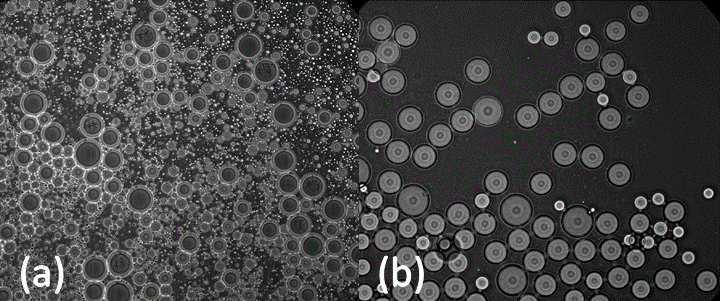
\includegraphics[width=\linewidth]{graphics/2025_09_28_droplets_fig3.png}
\caption{\textbf{Comparison of bulk droplets and on-chip droplets reveals broad size distribution in bulk droplets } In (a) we see bulk microdroplets after 21h of incubation (30$^\circ$C) without shaking. A broad distribution of droplet sizes can be observed. In bigger droplets, bacteria are observed. In (b), we see on-chip microdroplets. These are more uniform in size, especially a lower size limit can be observed and the bigger droplets are probably merged single droplets.}
\label{fig:results_droplet_bulk_vs_chip}
\end{figure}

\section{On-chip doplet production}

\section{Identifying producer-target pair}
After choosing our antibiotic producing strain, we used the well established halo-assay method to screen a collection of possible target strains, selected based on similar growth rate and easy culture conditions. We observe inhibition for several of the possible targets. Based on these results, we chose a \textit{Staphylococcus aureus} strain due to the large inhibition zone combined with its clinical significance. We ...

\begin{figure}
\centering
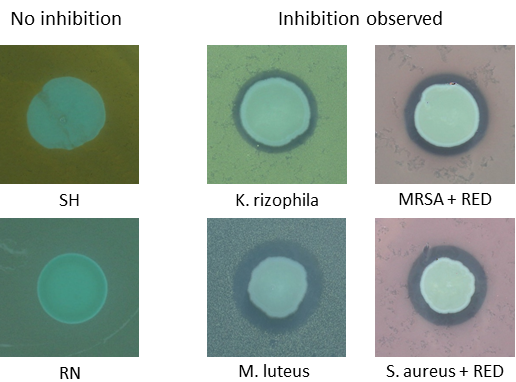
\includegraphics[width=\linewidth]{graphics/2025_09_28_droplets_fig4.png}
\caption{\textbf{Halo assay for library of target strains identifies \textit{S. aureus} as potential target} Using halo assays, we conducted a broad screening of very distinct bacterial strains to determine possible target strains for the chosen \textit{Bacillus subtilis} producer strain. Some natural isolates from our collection showed no inhibition but we observed several strains which exhibit inhibition. Among them the commonly used susceptibility test strain of \textit{Koccuria rizophila} but also clinically relevant strains of \textit{Staphyloccous aureus}, both methycillin-resistant (MRSA) and sensitive.}
\label{fig:results_sensitive_screening}
\end{figure}

\section{B. subtilis stressed in droplets}
After establishing the technical platform, we can incubate droplets for long periods of time and can monitor them under the microscope during these incubation periods.

\begin{figure}
\centering
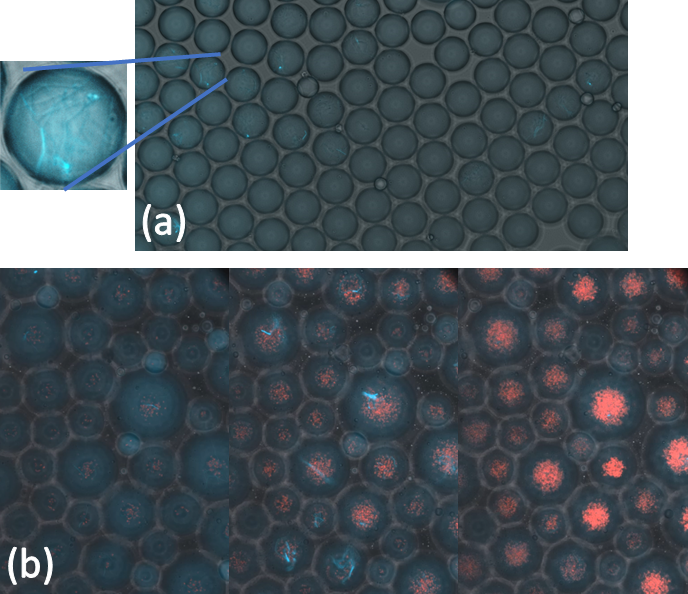
\includegraphics[width=\linewidth]{graphics/2025_09_28_droplets_fig5.png}
\caption{\textbf{On-chip droplets are stable after long-term incubation and allow bacterial growth} Our setup allows for long-term incubation and monitoring of droplets. (a) shows the results after 21h of incubation of droplets containing antibiotic producing bacteria alone in 30$^\circ$C without shaking. We observe stable same-sized droplets containing fluorescently tagged bacteria. The bacteria seem to be stressed and filament in the droplets. (b) shows snapshots of a time series of droplets containing both, antibiotic producing \textit{B. subtilis} (tagged in blue) and sensitive \textit{S. aureus} (tagged in red). Initially we see growth of both bacterial strains. However, \textit{B. subtilis} seems to be filamenting and at the end of the incubation, most droplets are filled exclusively with the target \textit{S. aureus} strain.}
\label{fig:results_incubation_subtilis}
\end{figure}

\section{Liquid vs. droplet comparison}
To understand if \textit{B. subtilis} disappears only in droplets or also in liquid, we performed a liquid-droplet comparison assay with separate cultures of B. subtilis and S. aureus. After incubation for 21h with high inoculation densities, we see that both liquid cultures exhibted growth while in droplets only the \textit{S. aureus} culture exhibits growth. The \textit{B. subtilis} culture in droplets seems to not support growth of bacteria.

\begin{figure}
\centering
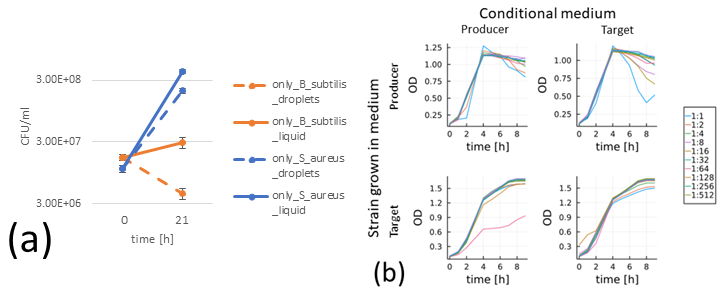
\includegraphics[width=\linewidth]{graphics/2025_09_28_droplets_fig6.png}
\caption{\textbf{\textit{B. subtilis} fails to grow in droplets and does not kill in liquid} To understand the observed dynamics in droplets, we conducted liquid experiments. (a) shows the results of comparing growth of antibiotic producing \textit{B. subtilis} in liquid and in droplets and similarly for the target \textit{S. aureus} strain. We observe that \textit{B. subtilis} seems to die in droplets while it grows in liquid culture. \textit{S. aureus} seems to grow almost equally well in droplets and liquid culture. (b) shows the results of growing bacteria in conditional medium. Studying every possible combination of producing and sensitive bacteria, we do not observe an effect of the antibiotic in liquid, hinting at the possible absence of toxic compounds in liquid compared to growth on solid media.}
\label{fig:results_liquid_vs_drop_supernatant}
\end{figure}

\section{Lack of antibiotic production in liquid}
Using an established conditional medium assay, we created a dilution series of the medium in which the producer previously grew. 